\chapter{Components}
\label{chap:components}

In this chapter we describe different frameworks and technologies, that we use (or could use as alternatives) in our system.
To build the complete Speed layer, we need several components.
First of all, message queue server receives messages from the outer sources, and feed them to the processing system.
Data processing system is the core of the system, and it stores results of computations in the data storage system.
Data storage system reliably keeps data in a distributed fashion. 

\section{Message Queueing}

Message queue servers are the important part of any data system.
They fill the gap between data sources and processing components or storage systems.
There are many message queue servers, here two of them - Kafka and RabbitMQ.
Additionally in this section we mention two serialization frameworks.
They tie different components of a complex system, written in different languages, together.

\subsection{Kafka [SP]}

The straightforward way to store user activity tracking data is to use a logging service.
It collects data, formes batches and stores them in a file system.
However, this approach does not provide a real-time access to stored information.
System that needs to handle real-time data cannot be content with batch-oriented mechanism.
It requires a pipeline that can transfer data between the system components without considerable delays.
Therefore a publish-subscribe mechanism named Kafka was invented by LinkedIn.

Kafka is a message broker that can deliver thousands messages per second. 
It provides high throughput and low latency of data handling.
It is built as a write-ahead log.
Data producers write data into a persistent store and data consumers read these records.
The Kafka structure is illustrated in Figure~\ref{fig:kafka_structure}.

The time of retaining a message is configurable.
The message is kept for a particular period of time, when it is available for consumption.
Then it is removed to free up space.

\begin{figure}[h]
  \centering
  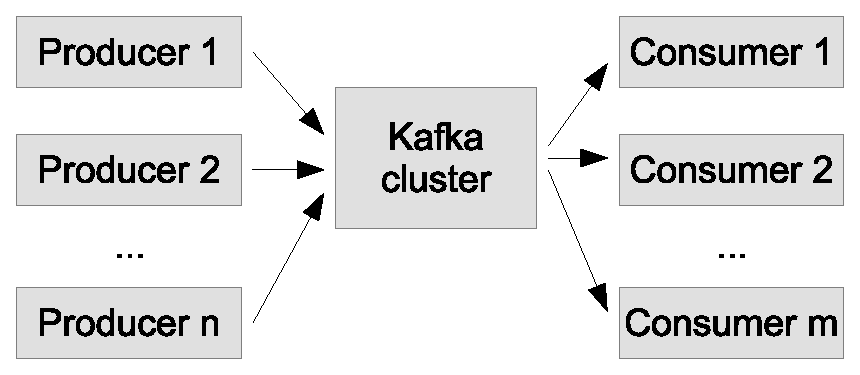
\includegraphics [width=0.5\textwidth]{images/kafka_structure}
  \caption{Kafka structure}
  \label{fig:kafka_structure}
\end{figure} 

\mnote{Kafka topic}
The core abstraction in Kafka is \textit{topic}.
One topic aggregates messages of one type.
For example, the system tracks the user activity, e.g. the number of times he opened a particular application or visited a particular website.
All these records are stored in the topic 'User activity'.
It is recommended to have a small number of topics (no more than a thousand).
However, each topic can contain  billions of messages.

One topic is a log that is spread over a cluster of brokers.
Every Kafka broker consists of zero or more partitions.
Figure~\ref{fig:kafka_topic_structure} illustrates the topic structure.
Kafka continually appends messages to the partitions.
Each partition represents an ordered sequence of messages that are uniquely identified by ids.
This id is called the \textit{offset}.
The sequence of messages is immutable and can only be extended by addition of new messages.
Besides appending, system provides one more operation: messages fetching.
Messages can be obtained from a particular partition, if a beginning message id is specified.
Kafka has an API for these operations, that can be used in different programming languages.

To provide fault tolerance, Kafka replicates each partition across several servers in a Kafka cluster.
One of these servers is a 'leader' and others are 'followers'.
The leader is responsible for handling all read and write requests.
The followers only replicate the leader.
For load balancing each server is simuntaneously a leader and a follower, i.e. for some of its partitions it acts as a leader and for others - as a follower.

The follower acts as a normal consumer, receiving data from the leader and applying it to its log.
Only when all the replicas received the message it is considered to be 'committed' and can be delivered to real consumers.
This guarantees that no message is lost even in the case of the leader failure.
A consumer always receives a message that is committed to the Kafka cluster.
A producer can wait until the message is committed or not, depending on the application logic.

To choose the leader, Kafka maintains a dynamic set of in-sync replicas (ISR).
Only these replicas can participate in the leader elections.
All these nodes must receive a message to consider it to be a committed write.
ZooKeeper stores the ISR set and tracks every change of its membership.
When a Kafka cluster has \textit{n}+1 replicas, it can sustain \textit{n} failures without any problems.

% �������� �������� ��� ��� � ������� ������ ����� ��� ���
%[reference: http://kafka.apache.org/documentation.html]
\begin{figure}[h]
  \centering
  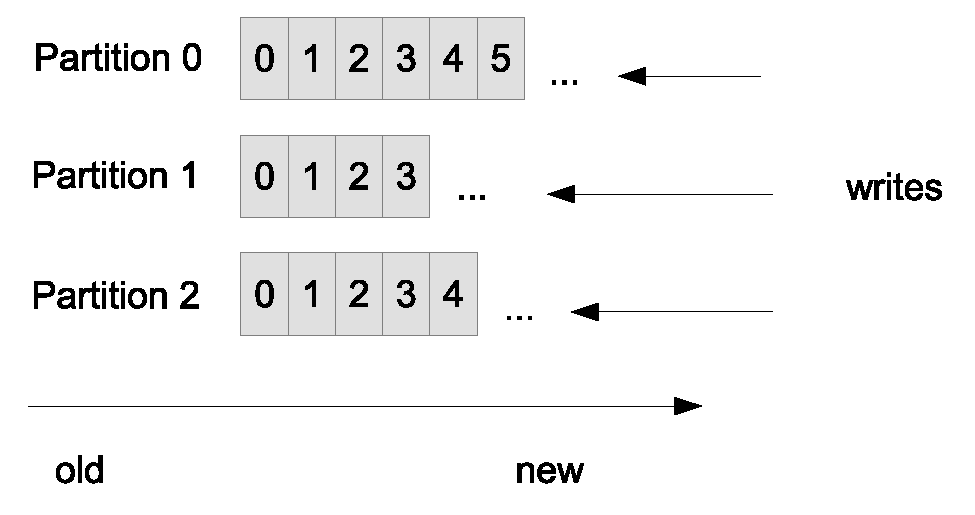
\includegraphics [width=0.5\textwidth]{images/kafka_topic_structure}
  \caption{Kafka topic structure}
  \label{fig:kafka_topic_structure}
\end{figure} 

Kafka uses a publish/subscribe mechanism to establish a communication process between producers and consumers of data.
One subscriber consists of a group of processes that run as a cluster.
Only one machine in this cluster obtains messages from Kafka.
Moreover, it consumes data from a specified partition.
Therefore, the subscriber parallelism depends on the number of partitions of the topic.
Kafka uses ZooKeeper to add or remove nodes from the broker and consumer groups.
It helps to rebalance the load automatically.

The fact that each partition has only one consumer makes it easier to store the metadata about what has been already consumed.
The consumer process just needs to store the last acknowledged message id.
Kafka uses 'at-least-once' semantic for message delivery.
It means that if the cunsumer process crashes, it reprocesses some messages from its partition one more time. 

There are two ways to balance load over Kafka brokers for message producers.
On the one hand, it can be done randomly.
On the other hand, application can supply a key that can be used to hash messages for partitioning.
The latter way guarantees the order of messages between partitions, that is not provided by Kafka.
Also it helps distributed consumers to make in-process aggregation.
In this case a consumer can obtain data from a particular partition, knowing that it contains a part of information it needs.  

For enhancing throughput Kafka introduces three techniques. 
First, it partitions data to production, consumption and brokering parts.
Second, it batches messages to chunks to send them together.
Third, it shrinks the data to decrease the amount of data that should be sent.

\mnote{batching}
The Kafka producer can send messages in synchronous or asynchronous ways.
In asynchronous mode small messages are collected into batches.
This allows to send data in chunks over the network. 
As it is done on application level, it is possible to control the batch size and the maximum time of holding the message.
Kafka allows to group messages from low-volume topics and high-volume topics together, reducing the amount of small requests.
On the filesystem level the mechanism of pagecache is used to buffer writes.
Kafka allows to delay the flush to disk again on the application level.
Similarly, it gives a control over the message boudaries and makes possible to have different policy for different topics.
Batching is also useful on the consumer side.
The client specifies the starting message id and the maximum buffer size it can receive at one time.
Kafka provides a possibility to combine data from several topics in one request.

\mnote{shrinking}
There are two techniques of data shrinking: via serialization and via compression.
Kafka associates schemas with the topics to extract the repeated structure from the messages.
Along with serialization, these schemas can be used to provide the compatibility and integration facilities.
The popular software that is used in combination with Kafka for serialization is Apache Avro.
It is described in details later in this chapter.
Kafka is able to compress several messages into a composite set of messages.
This is done during the batching process of the Kafka producer.
Thus, the messages in the compressed form are transferred to Kafka, where thay are stored and handled also in a compressed form. 

As the data transferred through Kafka is very diverse, a uniform schema is used for every topic.
This schema is kept all the way, from Kafka producer to Kafka consumer.
The schema usage is mandatory and is automatically checked.
As the schema sometimes changes, Kafka stores all its verions.
Each message contains a schema version id with which it was created.
Every schema is thoroughly tested when registered to detect incompatibilities in a timely manner.

\mnote{system monitoring}
A special Kafka topic exists to detect the percentage of data loss.
It audits the number of messages that are sent and received within a given topic over a specified period of time.
For this purpose each producer and consumer periodically notifies the audit topic about the number of processed messages.
The timestamps are extracted from the messages, instead of using the machine time of the message processing.
It is done to deal with delays in message delivering.
Kafka provides a standalone application for monitoring that processes the data from the audit topic.
It computes the ratio of data loss and duplication and is able to produce alert messages.

Kafka can by applied in a number of ways.
First, it can serve as a message broker, allowing to separate data producers from data processing.
Second, it provides facilities for real-time monitoring.
For instance, Kafka can be used to monitor the website users activity or to aggregate some application statistical data.
Third, it can serve as a log aggregation system, that can operate a log messages stream instead of dealing with log files.
This approach decreases latency and makes easier log data collection from several sources.

\mnote{log compaction}
One more Kafka application is a distributed system commit-log, that is used for restoring the failed nodes.
For this purpose Kafka has a specific feature - a \textit{log compaction}.
The main idea of log compaction is that Kafka guarantees that for all the message keys it retains the last known value.
The simpler data retention approaches are time- or size-based.
For example, Kafka removes the log data that is older than a specified period of time.
In this case some values that change rarely can be lost.
On the contrary, log compaction guarantees that at least the last value for each key persists.
This allows to fully restore the state of the broken node.

Another property of log compaction is that it shrinks the log size, removing the old records.
Using the complete log of all changes system can restore its state to any point by re-processing all the changes from the beginning of the log.
However, this approach requires a lot of memory for storing all the changes that leads to poor performance.
Log compaction removes only those records where more recent updates with the same key exist. 
Due to this fact the exterior system does not need to read the whole log and replay all the changes in order to restore its state.
Each topic has its own retention policy, i.e. one cluster can combine time or size retention with log compaction retention.

%[reference: http://kafka.apache.org/documentation.html#majordesignelements]
Figure~\ref{fig:kafka_log_structure} presents the Kafka log structure. 
The head of the log has a sequential numeration (offset) and retains all messages.
The tail of the log has a compacted structure, that contains only selected records.
It is important to mention that the messages in the log tail keep the original offset.
Kafka assignes this offset only once when a message is written for the first time and never changes it.
Moreover, even offsets for removed records are still valid log positions.
In this case Kafka returns the next highest existing value.
For instance, in our case requests with offsets 14, 15, 16 and 17 all return data starting from 17.

\begin{figure}[h]
  \centering
  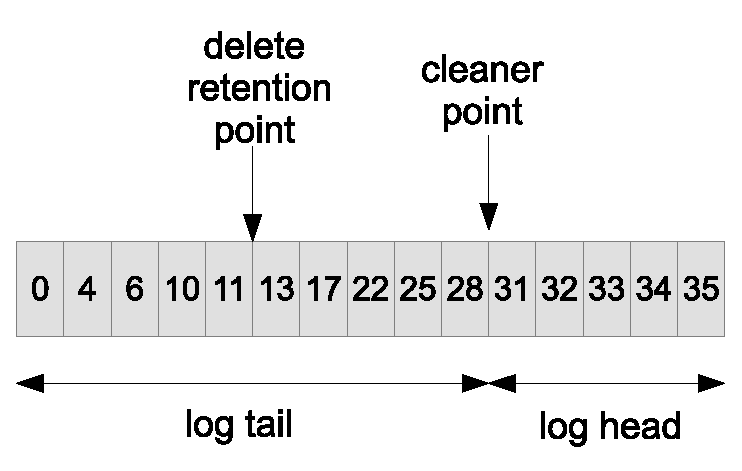
\includegraphics [width=0.5\textwidth]{images/kafka_log_structure}
  \caption{Kafka log structure}
  \label{fig:kafka_log_structure}
\end{figure} 

Compaction also performs message deletions.
If the message is marked to be deleted, all its previous versions (records with the same key) will be removed.
Deletion markers are not retained in the log after 'delete retention point' presented on the picture.

Log compaction is a background process that is run periodically.
Figure~\ref{fig:log_compaction_process} visualises a simple example.
Log compaction process posesses the following properties:
first, it guarantees the messages ordering even after compaction.
Second, the message offset is immutable and serves as a position of the record in the log.
Third, a read operation returns at least the final version for each value associated with a key.

\begin{figure}[h]
  \centering
  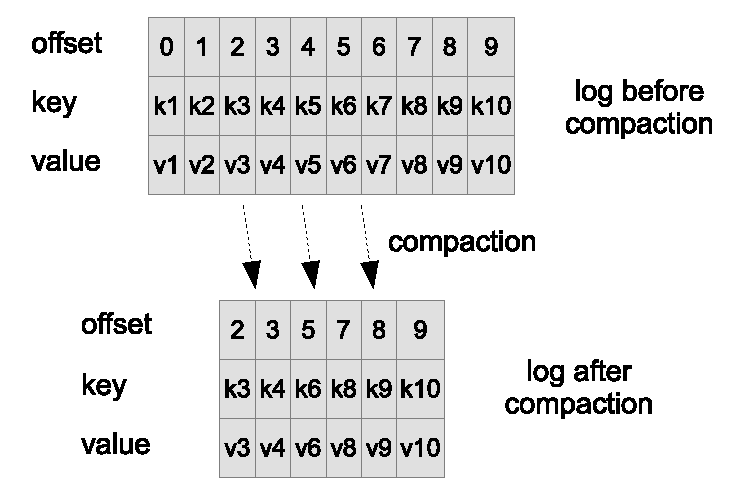
\includegraphics [width=0.6\textwidth]{images/log_compaction_process}
  \caption{Kafka log structure}
  \label{fig:log_compaction_process}
\end{figure} 

The compaction process consists of the following steps:
(1) The log is chosen, that has the biggest number of records from log head to log tail.
(2) For each key in the log head compaction process determines the last offset.
(3) The log is copied from the beginning to the end, removing the keys that occure later in the log. 
   



\subsection{RabbitMQ [VI]}

RabbitMQ is a queue messaging server \cite{RabbitMQ, AlvaroWilliams2012}.
It provides a robust, efficient and scalable message broker, that serves as an intermediate layer between publishing and subscribed clients.
RabbitMQ has a simple data model, that nevertheless offers a flexibility in the structure of data flows.
It gives an opportunity to adjust a tradeoff between throughput and reliability.
RabbitMQ fully applies Advanced Message Queuing Protocol (AMQP).

General structure of RabbitMQ
Producers
Consumers
Brokers
AMQP connection and channels

\textit{Advanced Message Queuing Protocol} \mnote{Advanced Message Queuing Protocol (AMQP)} or \textit{AMQP} is something \cite{AMQP2011}.

Queues

Exchanges and bindings
Routing key and exchange type
Direct
Fanout
Topic

Virtual hosts and separation

Durability
Delivery mode - persistent
Durable exchange
Durable queue

Delivery verification
\subsection{Avro [SP]}
\label{subs:avro}

Data should be structured when it is transferred over the network.
Data objects are converted into some form, in which they can be stored or transferred and later be reconstructed in a new environment.
This process is called serialization.
The naive serialization approaches are XML or JSON.
Drawback of these formats is that they require too much space for storing, because the data is kept it a text form.
The better solution is to use binary format for serialization and Apache Avro is one of the frameworks that use such approach.

Avro differs from the other serialization frameworks in that it does not require the code generation on receiving \cite{Avro1}.
It even allows to efficiently sort binary-encoded data without deserialization.
Also Avro supports easy schema changes, because it stores both old and new schemas and can associate fields with each other using their names.
This framework provides two types of encoding: binary encoding and using JSON.

Avro uses \textit{schemas} that are defined using JSON.
It needs a schema for serialization and in most cases this schema is transmitted along with the data.
Thus the receiving application does not need to store schemas for deserialization.
However, in some scenarios the transmission of schema is redundant, because both sides have the full schema stored locally.
In this case it is possible to transmit only a binary representation of serialized objects.

The schema can contain both primitive and complex types.
Primitive types include: \textit{null}, \textit{boolean}, \textit{bytes}, \textit{int}, \textit{long}, \textit{string}, \textit{float} and \textit{double}.
Complex types are: \textit{record}, \textit{array}, \textit{enum}, \textit{union}, \textit{map} and \textit{fixed}.
Listing~\ref{lis:example_avro_schema} illustrates the example schema.
One schema files stores only one schema definition.

\begin{lstlisting}[caption=Avro schema (example), label=lis:example_avro_schema]
{
  "name":"AppInstall",
  "namespace": "example.avro",
  "type":"record",
  "fields":[
     { "name":"id", "type":"long" },
     { "name":"userId", "type":"long" },
     { "name":"time", "type":"long" },
     { "name":"appName", "type":"string" },
     { "name":"packageName", "type":"string" }
  ]
}
\end{lstlisting}

Avro uses an \textit{object container format} for storing objects in a file.
A file has a specified schema, that consists of blocks with synchronization markers between them.
Blocks contain data objects and can be compressed.
Synchronization markers allow to split file for processing it with MapReduce.
Moreover, Avro file contains metadata section, where it stores a schema.

A file has the following structure: it has a header and one or several file data blocks.
The header contains information about encoding type and file metadata.
Metadata stores the schema and a type of codec that is used for compressing.
'null' codec type means that the data is uncompressed, 'deflate' codec uses the deflate algorithm.
The file data block stores information about the number of objects it contains, their sizes in bytes after compression, the serialized objects themselves and a synchronization marker.
This additional data helps to detect corrupted blocks.

Avro provides a \textit{Remote Procedure Call} (RPC) interface for implementing data exchange between a server and a client.
RPC protocol is defined using JSON.
Its attributes include a \textit{messages} object, that specifies the messages that are exchanged.  
\textit{Message} is a byte sequence, that is transmitted using a transport mechanism.
Transport system sends requests and receives responses.

Transport can have a stateless or stateful design.
\textit{Stateless} means that a server does not store any information about a client state.
The client transmits all the needed data in every request message.
In \textit{stateful} design the server keeps the persistent client state.
This approach has two problems.
First, the server should have a mechanism to discard client state at some point.
It is not possible to store the states of all the client for unlimited period of time.
Second, the server should be able to restore the client state in the case of the server crash.
This makes the process of server-side implementation complex comparing to sateless design.
However, stateful design results in better performance.
Figure~\ref{fig:stateful_stateless} represents the stateful and stateless schemas.

\begin{figure}
  \centering
  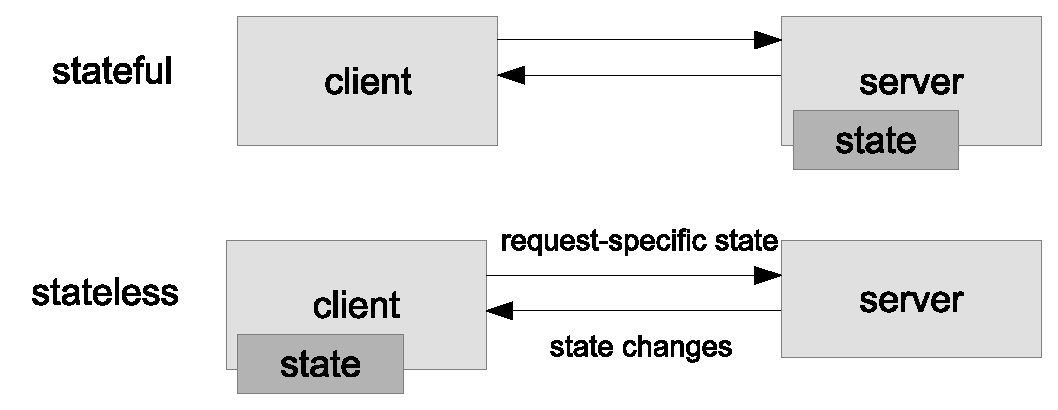
\includegraphics [width=0.7\textwidth]{images/stateful_stateless}
  \caption{Stateless and stateful design}
  \label{fig:stateful_stateless}
\end{figure}

An example of stateless transport method for Avro is HTTP.
In this case all Avro messages share the same URL at an HTTP server.
The 200 (OK) response code should be used by all response messages (normal and error).
Avro sends requests via the POST method.

There is an intermediate layer between messages and transport named \textit{framing}.
The main idea of framing is the partition of each message to a list of buffers.
A buffer contains buffer length followed by buffer data of this length.
Every message consists of one or several buffers.
Framing makes read and write operations more efficient.

Avro uses a handshake procedure before sending any RPC requests and responses.
It is used to make sure that the protocol definition is the same on both the server and the client side.
Only in this case the server and the client can correctly deserialize requests and responses.
To avoid extra network exchanges the server and the client stores recently used protocols in a cache.
Stateless and stateful transport differs in that the former requires a handshake before every request and response.
In contrast, the latter needs only one handshake and for the lifetime of the connection.

The handshake procedure is the following.
The client sends a \textit{HandshakeRequest} in a form \textit{(clientHash=clienthash, clientProtocol=null, serverHash=serverhash)}.
The \textit{clienthash} and the \textit{serverhash} are both the JSON protocol text, hashed with MD5.
The \textit{serverhash} contains data that the client received from the server during the last session.
If it is the first connection to this server the client tries to guess the server's hash.
The server sends in response a \textit{HandshakeResponse}.
If the received \textit{serverhash} is valid and the server knows the corresponding protocol to this client, the response has a form \textit{(match=BOTH, serverProtocol=null, serverHash=null)}.
In this case the connection is confirmed and the server can send a response message.
If the \textit{serverhash} is not valid, but the server knows the client protocol, it answers with \textit{(match=CLIENT, serverProtocol=serverprotocol, serverHash=serverhash)}.
It also allows the server to send the response data to the client.
However, the client must replace its nonvalid \textit{serverhash} data with that received from the server and process the response using the received protocol.
When the server is not aware of the client's protocol it received, it response with \textit{(match=NONE)}. 
Then the client re-sends its request extended by \textit{clientProtocol} value and the server response with \textit{(match=BOTH)}.

To determine the identity of the schemas stored on the client and the server side, Avro uses \textit{Parsing Canonical Form}.
It is a transformation, that removes data, irrelevant for the comparison, and normalizes the JSON text.
This canonical form can be used to create a fingerprint (an integer that serves as a unique id for a schema). 

 


\subsection{Thrift [VI]}

Description of Thrift \cite{Slee2007} \cite{Thrift}.



\section{Real-time Data Processing Systems}

Efficient processing of big volumes of data is a crucial point for any big data system.
It must be easy to model, develop and maintain.
This section describes two data processing frameworks - \textit{Storm} and \textit{Spark}.
They have different computational models, but allow execution of the same computations.
The difference between them is that Storm is a truly real-time processing system, whereas Spark works essentially with batches, and has a streaming extension on top of batch computations.

\subsection{Storm [SP]}

Batch processing is not applicable for real time computing.
Hadoop, the best known tool for batch processing, is helpless when it is needed to handle streaming data and obtain immediate result.
The main advantage of real time processing, the guaranteed time delay between a request and a result can be broken simply because the waiting time for the next batch is too long.
Therefore new systems, designed for real-time processing, have appeared.
One of such systems is an open source project named \textit{Storm}.

Storm is a \textit{complex event-processing} (CEP) system.
Complex event processing means gathering data from different sources, combining it and making conclusions from it.
For example, such system keeps track of significant changes in traffic reports or stock market feeds and immediately responds to them. 

Storm is implemented in a dialect of the Lisp language named Clojure.
Clojure is a functional language like Lisp, but it also supports multithreaded programming.
Clojure runs on the Java Virtual Machine, however applications within Storm can be written in Java, Scala, JRuby, Perl and PHP.
Moreover, one can use a Structured Query Language adapter for streaming data directly into Storm topoloy.

\mnote{Storm architecture}
The Storm cluster has a master node called \textit{Nimbus} and \textit{worker} nodes.
Nimbus assignes tasks for workers and monitors failures.
There is a deamon called \textit{Supervisor} on every worker node.
The supervisor is responsible for starting and stopping worker processes assigned by Nimbus.
ZooKeeper coordinates the interaction between Nimbus and Supervisors.
It stores the state of all the nodes, making the system stable to failures.
If any of the nodes is killed, ZooKeeper immediately restarts it, enhancing Storm cluster stability.
ZooKeeper is described in more details later in this chapter.

The basic concept of Storm is a \textit{topology}.
It is a graph of computation, that shows how data should be processed and passed between the nodes.
One can implement a topology in any programming language, because topology definition is a Thrift structure.
Thrift is a framework that allows to develop cross-language services.	

The data stream consists of an unbounded set of \textit{tuples}.
A tuple can contain both standard data types (integer, float, byte array) as well as user-defined types.
Every stream has its own ID.
The sources of streams called \textit{spouts}. 

The next important Storm primitive is \textit{bolt}.
Figure~\ref{fig:storm_architecture} shows the interaction between spouts and bolts.
The stream of tuples originates from a spout and goes through a sequence of bolts.
Every bolt performs a transformation on incoming data stream, like aggregating, filtering, or interaction with external parts such as databases.
A bolt can receive information from several spouts and stream it to multiple bolts.

\begin{figure}
  \centering
  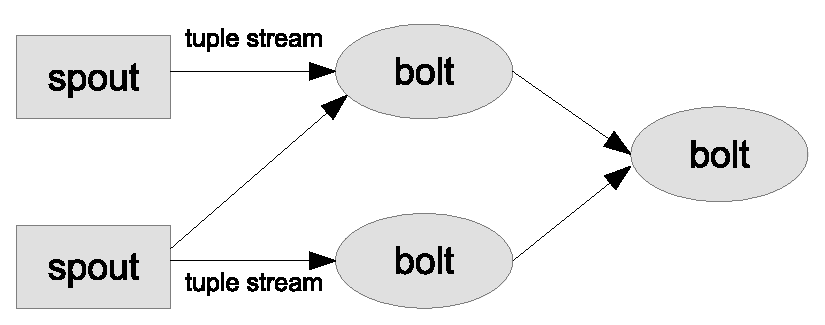
\includegraphics [width=0.5\textwidth]{images/storm_architecture}
  \caption{Storm architecture}
  \label{fig:storm_architecture}
\end{figure}

For example, MapReduce word counting example can be easily implemented with Storm.
Such system counts how many times each word occures in a given input data.
In the case of Storm one needs 
(1) a spout to generate text data, 
(2) one bolt to implement the Map function for word tokenisation and 
(3) one bolt to implement the Reduce function for aggregation the amounts of words occurences. 

Storm allows to group the stream of tuples in different ways.
For instance, shuffle grouping randomly distributes tuples to bolts such as each bolt receives approximately the same number of tuples.
Field grouping partitions tuples according to contained fields.
Also other grouping methods exist, including the custom grouping.

The Listing~\ref{lis:simple_storm_topology} represents a simple topology.

\begin{lstlisting}[caption=Simple Storm topology, label=lis:simple_storm_topology]
java TopologyBuilder builder = new TopologyBuilder();
builder.setSpout("myspout", new TestSpout(), 10);
builder.setBolt("mybolt1", new TestBolt(), 3) .shuffleGrouping("myspout");
builder.setBolt("mybolt2", new TestBolt(), 2) .shuffleGrouping("mybolt1");
\end{lstlisting}

Here topology consists of one spout and two bolts.
The stream of tuples originates from \textit{myspout}, then it is passed to \textit{mybolt1} and finally to \textit{mybolt2}.
In both cases tuples are grupped using the schuffle grouping method.
The integer numbers in \textit{setSpout} and \textit{setBolt} define the amount of parallelism for the node.

The implementation charasteristics of Storm lead to high performance and guaranteed fault tolerance.
It uses ZeroMQ for passing messages between the tasks.
Messages are automatically serialized and deserialized to Storm primitive types.
The usage of this message queue helps to avoid intermediate queueing, thus improving performance.
Furthermore, Storm guarantees the processing of every tuple.
In the case of a fault during message processing, a tuple is replayed from the spout.
There is also a fault detection mechanism on task level, when the failed task is quickly reassigned to restart the processing.
Storm has supervisors to manage the processes, that leads to efficient usage of resources.

Storm cooperates with message queue systems in such a way that every message is fully processed.
It builds a tuple tree, that reflects the motion af all the tuples.
Only when every message in the tuple tree is processed, a tuple is considered to be fully processed.

To give an example, let us take a message queue that supplies a spout with messages.
When the spout takes a message from the queue, the message state changes to 'pending'.
In this state it cannot be sent to other consumers.
Moreover, all the messages in pending state are returned to message queue if their consumer disconnects.
Storm assignes a unique id to the message, if it is not given by the message queue.
Using this id Storm can keep track of this message during processing.
The system receives this message when the \textit{nextTuple} method of the spout is called.
The spout emits the message along with its id to the consuming bolts.
When a tuple is fully processed, the \textit{ack} method of the original spout is called. 
In the case of time-out Storm calls the \textit{fail} method of the same spout.
Only when \textit{ack} or \textit{fail} method is called, the spout sends an ack or fail message to the message queue.
The message queue cancels the pending state of the message, taking it off the queue in the case of success and putting it back otherwise.

Storm can process not only the tuple trees, but also directed acyclic graphs.
It happens when an output tuple is anchored to several input tuples.
\textit{To anchor} means to specify a link in the tuple tree.
Multi-anchored tuples often appear during streaming aggregation or joining.
 
As it was mentioned, Storm tracks every tuple using its unique id.
Additionally, as each tuple exists within a tree, it knows all the tuples ids of this tree.
For example, if a bolt emits a new tuple, this tuple carries the ids of spout tuples received by this bolt along with its own id.
Such storage mechanism is used	because when the tuple is acked or failed, it should inform Storm about its dependencies to restore the state of the tuple tree.  

The acker task is responsible for acking the tuple.
First, Strom stores the mapping between an acker task and a spout tuple id.
As every tuple keeps ids of spout tuples in the tree it exists within, it knows the acker tasks it should communicate with.
A tuple informs an acker task when the tree is fully processed and the tuple is acked.
Second, the acker task should send a complition message to the spout task that emitted this tuple.
For this purpose, on creation of a new tuple a spout task notifies the appropriate acker task that its task id is linked to that spout tuple.

For acker task tracking the huge tuple trees explicitly is not efficient.
Thus Storm uses a special tracking strategy.
An acker task stores a map: on the one side it has a spout tuple id and on the other side a pair of values.
One of the values is a task id the spout tuple originates from, and the other is an 'ack val', the 64 bit number.
The 'ack val' represents the state of the tuple tree without storing it in memory.
This number is a result of XOR operation on all created and acked tuple ids of the tree.
Therefore, when the 'ack val' is equal to zero, it means that the tree is completed.
\subsection{Spark [VI]}

Spark is a framework for distributed data processing \cite{Zaharia2010} \cite{Zaharia2013} \cite{Spark1} \cite{Spark2}.
It provides a tool to work with large datasets and streams of data, and to make complex queries on this data.
Spark has several abstractions for representation of data and streams.
The first one - Resilient Distributed Dataset (RDD) - is an object, distributed in the cluster, that contains data to process.
Another one is a Shared Variable - variable, that can be used among the cluster as a counter or lookup table.
One more abstraction is a Discretized Stream (DStream) - representation of a data stream also in a distributed fashion.

\subsubsection{Data model and batch processing}

To initialize Spark you first create a SparkContext object, that is responsible for a connection of your program to Spark.
It allows to specify properties of your application, and also options of how Spark should run, for example in local mode or on the cluster.
SparkContext gives an access to different parameters and properties of execution environment.

\textit{Resilient Distributed Datasets}\mnote{Resilient Distributed Datasets} (RDDs) is a main abstraction in Spark, that represents dataset in a distributed fashion.
RDD is essentially a readonly collection of elements.
It is fault-tolerant, so that if one partiotion is lost, the whole collection can be recovered.
RDD does not need to exist physically on the cluster nodes.
Instead, it is a lazy object, that can lay in a robust data storage, and be computed on the fly, when computations require particular pieces of data.

There are two methods how to obtain an RDD object: parallelizing exisiting collection in the driver program, and using external dataset.
Existing collection is any collection of data, e.g. array, list, set, etc., that you in fact have in the program.
When you create an RDD object in this way, elements of a collection are copied to a distributed dataset, that you can use than in parallel.
You can specify the number of slices, that is the number of tasks, each machine in the cluster will then execute for this collection.
External dataset is an external file.
It can reside in the local file system, and in the distributed file system like HDFS.
The simple example of what you can do with the external text file, is to count the sum of lines' lengths using functions $map$ and $reduce$ of an RDD object. 
Additionally, you can obtain RDD by transforming another RDD, or by changing persistance of an existing RDD, but this methods are derived in some sense.

RDD supports two types of operations: \textit{transformations} \mnote{transformation} and \textit{actions}\mnote{action}.
Trnsformation creates a new RDD object from existing one.
An example is a $map$ function, that processes each element of an RDD object using specified function, and returns a new RDD object as a result.
Action executes computations on an RDD object, and returns a value.
$Reduce$ is an example of action.
It aggregates all elements giving in the RDD object and return the resulting value.

Transformation in Spark is a lazy operation, in the sense that it is computed only when action operation requires its result to produce output.
This makes execution more efficient when there is a chain of transformations before final action, because your application does not receive then intermediate RDD objects, but only final resulting value, that is usually much smaller.
Nevertheless, there are cases, when you want to compute different actions on the same transformation.
Then it is meaningful to have RDD object of this transformation computed once, and to have a handle to it in your program.
For this case there is a method $persist$, that allows to materialize RDD object.
This is also possible to persist RDD object on disk.

Next we present a simple program, that counts the sum length of all lines in a text file:
\begin{verbatim}
JavaRDD<String> lines = sc.textFile("data.txt");
JavaRDD<Integer> lineLengths = lines.map(s -> s.length());
int totalLength = lineLengths.reduce((a, b) -> a + b);
\end{verbatim}
Example is taken from \cite{Spark1}.
Here we create an RDD object from external file, set $map$ function to count length of the line, and set $reduce$ function to sum up lengths of lines.
Execution starts only when $reduce$ function is called, because, as we discussed, transformations are lazy in Spark.

Normally, when you pass arguments to any function, that executes on the nodes of the cluster, they are simply copied and there is no feedback to the driver program.
Sometimes it is useful to have global variable or lookup table, that all nodes can access.
Spark supports the notion of \textit{shared variable}\mnote{shared variable}.
There are two types of shared variables: \textit{broadcast variables} \mnote{broadcast variable} and \textit{accumulators}\mnote{accumulator}.
Broadcast variable represents readonly value or dataset, that is useful for all nodes as a lookup table or global predefined value.
It is copied to every node using method $broadcast$ of $SparkContext$.
There are efficient algorithms in Spark to make this transfer fast.
Accumulator is distributed counter, that allows all nodes to add up to the global numeric variable.
It can be created using method $accumulator$ of $SparkContext$.
No node can read this value or do anything else than incrementation, what makes its implementation easy and fast.
Only driver program is able to read accumulator's value.

\subsubsection{Streaming processing}

Streaming in Spark is an extension of a Spark engine, described in the previous section.
It can process data stream in a distributed manner.
Spark Streaming receives data from the input stream, divides it into blocks, each represented as an RDD, and passes this sequence of blocks to the Spark engine.
It can work with different sources, e.g. message queue server (Kafka), web service (Twitter API), or regular TCP socket.
Processed data can be there stored to the filesystem or database.
The main abstraction for streaming processing in Spark is a Discretized Stream or DStream.
It is internally a sequence of RDDs.
Several DStreams can be combined into one chain for application more complex algorithms. 

Similarly to Spark engine, you must create $SparkStreamingContext$ object to work with Spark Streaming.
It allows to adjust environment for processing, set properties like local or cluster mode, number of threads used, and many others.
One important propery is the batch interval.
It defines the time of gathering data from the input stream, before creating DStream and sending it to the Spark engine.

\textit{Discretized Stream} \mnote{Discretized Stream (DStream)} or DStream is the main abstraction in Spark Streaming.
DStream can be the input stream, as well as intermediate stream, generated after processing of input stream of data.
It is essentially a chain of RDD objects, and provides a stream of data, that is to process by Spark.
Each RDD represents batch of data in the period of time, that is specified in the $SparkStreamingContext$.
Figure~\ref{fig:SimpleDStream} depicts simple DStream.

\begin{figure}[H]
  \centering
  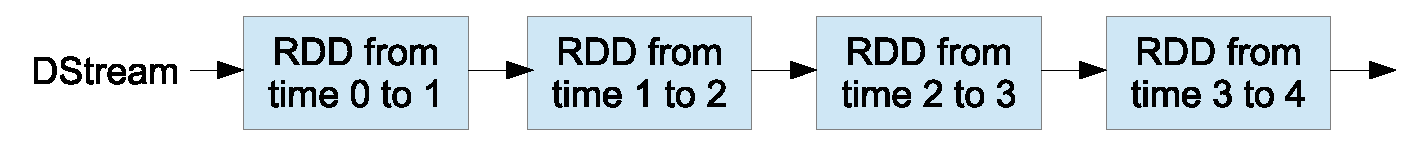
\includegraphics [width=1.0\textwidth]{images/SimpleDStream}
  \caption{Representation of a simple DStream.}
  \label{fig:SimpleDStream}
\end{figure}

Every operation you want to apply to DStream is applyed to every RDD object in the stream.
This implies, that transformation on the DStream produces new DStream.
All these transformation are executed by Spark Engine in a standard batch fashion.
Figure~\ref{fig:DStreamWithTransformation} depicts how it works.

\begin{figure}[H]
  \centering
  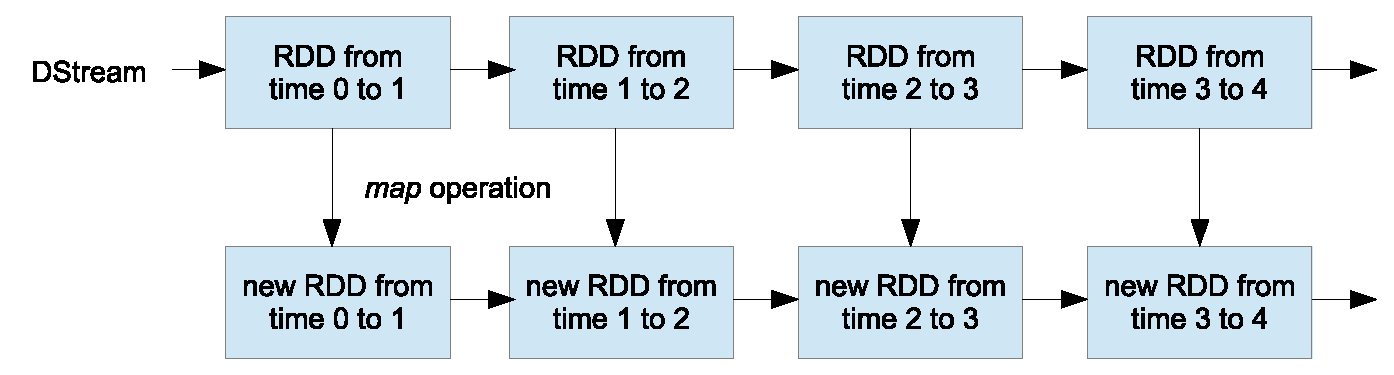
\includegraphics [width=1.0\textwidth]{images/DStreamWithTransformation}
  \caption{Transformation of a DStream to a new DStream.}
  \label{fig:DStreamWithTransformation}
\end{figure}

\textit{Input DStream} is a stream of raw data coming to Spark from the outer source.
Sources can be of two types: basic sources and advanced sources.
Basic sources are sources, that available using standard streaming context API, e.g. files or sockets.
Advanced sources are available using specific libraries, for example Kafka message queue server.
There is a notion of $Receiver$, that is an object that receives data from the stream, put into Spark's memory, so that it is available for input DStream, associated with this Receiver.
Every DStream is responsible only for one input data stream.
You can create many DStreams for different input streams to receive data from different data sources in parallel.
Receiver is executing as a long running task, hence it occupies one core of the processor.
This implies, that there should be more cores then receivers in the system.

Transformations on DStreams (UpdateStateByKey Operation, Transform Operation, Window Operations) ???

Spark streaming has a number of output operations on DStreams, that used to push transformed data to outer systems.
This can be files or databases.
Output operations actually start execution, as $actions$ of Spark engine do.
Examples of output operations are $print$, $saveAsObjectFiles$, $saveAsTextFiles$, $saveAsHadoopFiles$, $foreachRDD$.

DStream allows to persist it in the memory, when multiple computations of the same DStream are required.
Method $persist$ of DStream object does that.
Its execution specifies that every RDD of the DStream will be persisted in the memory, as it is done for RDD in Spark engine.
For data, arriving from network, the persistence level is so, that all data is replicated to two nodes to provide fault-tolerance.

There is a mechanism of checkpointing in Spark streaming.
It allows to make snapshots of intermediate data to HDFS.
It makes computation throughput less, if set not properly.
So it must be carefully tuned.

Fault-tolerance of Spark streaming is based on the fault-tolerance on Spark engine.
RDDs are basic elements of a DStream, what lets Spark streaming to rely on their robustness.
As long as all data locates on HDFS, if data node fails, all lost data can be recovered.
For data coming from network input stream, as we already mentioned, it is always replicated to two nodes.

\section{Storage Systems}

There are nowadays many different storage systems for big data management.
They have different data models and, hence, different applications.
Often they store data in a key-value manner.
In this section we consider three systems that are relevant for our work.
HDFS is a distributed file system that keeps data essentially in a tree structure in files.
Redis is a very simple in-memory key-value store.
Cassandra is more sophisticated column-style fully distributed data storage.

\subsection{HDFS [VI]}
\label{subs:HDFS}

The Hadoop Distributed File System (HDFS) is a distributed data storage that provides high throughput data access, fault-tolerance, ability to hold big datasets consisting of large files \cite{HDFSArchitecture1, HDFSArchitecture2}.
The Apache Software Foundation has developed HDFS originally for its web search engine - the Apache Nutch.
Today it is a widely-used distributed file system, that is an infrastructure for such distributed computational frameworks as Hadoop, Storm, etc.
HDFS allows to use cheap commodity hardware, because it does not require much computational or storage power for one particular node.
It is written in Java, hence, any platform with JVM \cite{JVM} can run HDFS's software.
HDFS supports standard hierarchical file organization with directories and files.

%\subsubsection{Use cases and requirements}

HDFS provides high throughput data access, because it is designed for usage in the BigData world.
Applications, that use HDFS, require fast writing and reading of files of gigabytes and terabytes in size.
HDFS is suitable for the batch processing, and it is important to say, that low-latency is not a goal property.
It allows to operate with the large number of files.

Fault-tolerance, detecting of failed machines, and recovering from inconsistent state of the file system are inherent properties of HDFS.
This is a key property, because disk failures and machine failures in general, happen more often, than we could think.
When we consider a cluster of hundreds and even thousands of nodes, this is actually a normal case.
Google has made a deep research on this topic, and has found out that 8\% of hard drives fail in two years \cite{Pinheiro2007}.
This statistic shows that it is reasonably expected that in the large cluster there are always machines that are out of service.

HDFS has a simple file storage model.
It holds every file in a coherent way, so that it can be only written, and not changed any more.
Only one client writes the file to the file system, but many clients can then read it.
This model has a name \textit{write-once-read-many}, and it helps to provide high throughput data access.

HDFS lets an opportunity to move computations into the cluster, instead of moving data from the cluster to where computations are executing.
This is proven to be much more efficient, because moving data creates high network congestion.
When the data is of a very high volume it is important aspect to consider.

HDFS is written in Java, what allows to run it on practically all platforms and any hardware.
The only requirement for a machine to use it in the HDFS-cluster is that it has running JVM.

%\subsubsection{General structure}

HDFS consists of two main elements: NameNode and DataNode.
These are applications that run on JVM.
They both do not require any particular operational system or hardware, and use local file system for storage of HDFS data pieces.

NameNode is a master program of the cluster.
It stores meta information about the file system's namespace, regulates access of the clients to files, maintains consistent state of the file system, initializes operations like create, rename or delete file.
NameNode is of the highest importance, because its failure can be dangerous for the whole system.
It runs usually on a special separated machine.
The fact that there is only one master node greatly simplifies system's structure, its maintenance and analysis of errors.
Data never flows through the NameNode.

DataNode is a program that holds data.
Each machine in the cluster runs usually one DataNode.
DataNode executes read and write requests directly from the clients.
It also performs creation, deletion and replication of blocks, when NameNode gives such instructions.

DataNodes hold files in blocks.
Standard size of a block is 64 Mb.
Normally, each block resides on the different DataNode to provide high reading throughput.
Every file has replication factor, that defines the number of its replicas.
If replication factor is for example 3, than each block of this file has 3 copies on different machines.
This provides fault-tolerance in case of disk or other hardware failures.

Applications access HDFS using Client program, that provides interface to do write and read requests.
When Client writes, it asks NameNode to give a list of DataNodes to write replicas of the first block.
Then it accesses DataNode directly and makes write of the block.
DataNode in its turn sends write request of this block to another DataNode, that is in the list for replications.
And so on, until the block has all its replicas written.
When block is written, Client asks about new list of replicas for the next block.
When Client reads, it asks NameNode for the list of replicas of the first block, sorts it by the distance in the network topology, and then gets it from the nearest replica.
Then the same for the next block and so on.
You can see the overall structure of HDFS and the way of its functioning on the Figure~\ref{fig:HDFS}.

\begin{figure}[h]
  \centering
  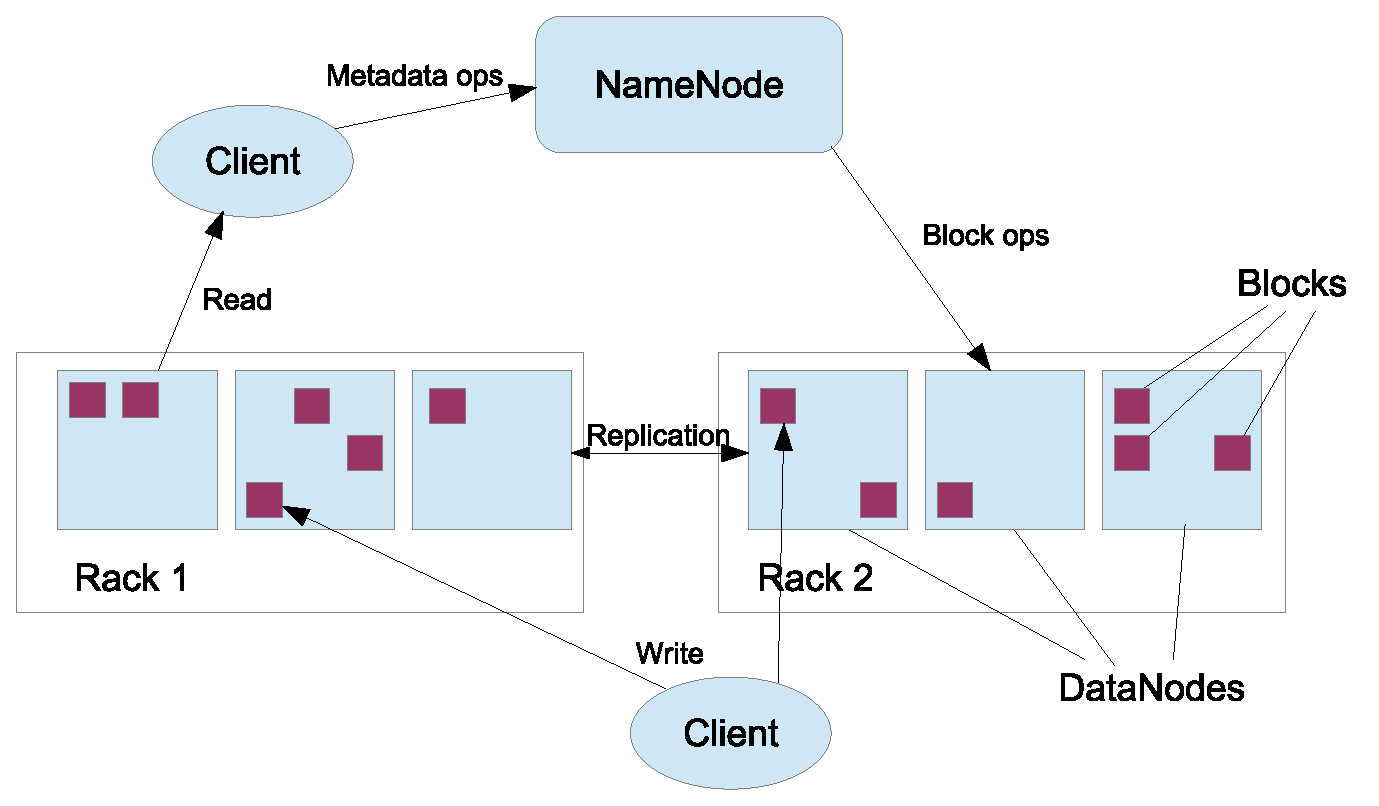
\includegraphics [width=0.8\textwidth]{images/HDFS}
  \caption{Overall structure of HDFS.}
  \label{fig:HDFS}
\end{figure}

%\subsubsection{Replications}

HDFS stores large files reliably, so that failures of particular machines can lead to an unrecoverable loss of a part of a file with a very small probability.
It also provides high throughput, placing blocks of files onto different DataNodes, to give parallel access of many clients to many files in the cluster.
The number of replicas and the block size are configurable parameters for every file.
Replication factor also can be changed for already existing files.

Cluster consists of the number of racks.
Rack is a group of nodes, that reside usually near to each other physically.
This helps to avoid redundant network usage, and to make replication algorithms more efficient.

The current replicas placement policy for the most common replication factor of 3 is as follows.
Put the first replica onto the DataNode in the rack, local for accessing client.
Put the second replica in the same rack, but onto the other DataNode.
Put the third replica onto the DataNode in another rack.
This approach gives both high fault-tolerance and near to optimal access rate.

%\subsubsection{Robustness}

One of the main goals of HDFS is to provide fault-tolerance from hardware failures.
For this sake, each DataNode sends periodically a Heartbeat signal to the NameNode, to notify about its state.
If the DataNode's machine fails, the NameNode does not receive Heartbeat signal, and marks this DataNode as out of service.
The NameNode starts then re-replication of blocks, that resided on the failed machine.
Another condition to make re-replication is increase by the client of the replication factor of a particular file.

When the piece of data arrives to the client, it can be corrupted during transfer in the network or because of a IO failures.
To provide integrity of data, HDFS has a checksum mechanism.
When a block of file is written, its checksum is also written to the file system.
Then, when client reads a block, it also receives checksum and able to match block.

HDFS manages balance in the cluster.
If there are DataNodes that has free space below set threshold, file system moves part of data from that nodes to others, that have more free space.
This is done automatically, and does not allow to accumulate data in the part of the file system, decreasing its access throughput.

There is a staging mechanism in HDFS, that helps to avoid network congestion.
Client, that writes data to the file system, does it in portions.
It accumulates the whole block in the local cash file, and only then makes flush to the DataNode.
\subsection{Redis [VI]}

Redis is an open source key-value in-memory data storage \cite{Seguin2012} \cite{Redis}.
It affords blazingly fast and simple tool for maintaining data inside of a single application or a cluster.
Redis is very easy to deploy, learn and use.
It provides 5 data structures, e.g. string, list, set, ordered set and hash, that are useful for different tasks, and give a powerful tool in combination.

\subsubsection{Basics}

Redis is a key-value store, that allows to hold all data of your application.
Redis lets to create many databases and switch between them.
For one database it maintains one global map of keys to values.
Although Redis is in-memory database system, it swaps data continuously to disk to provide persistance in case of application's failure.
This is also important in a distributed environment to have global data available between applications.

Record in Redis is a key-value pair.
The key is always a string.
It does not contain data, that your application manipulates, but it identifies piece of data, that you want to store.
The value can be of different types, but in any case it is a meaningful peace of data, that you store in the database.

Redis provides many useful and at the same time simple commands to work with data.
The two simplest commands are $SET$ and $GET$, that let to store a key-value pair into database, and to get value by key, respectively.
This is an example of how you can use these commands:
\begin{verbatim}
> SET server:name "SERVER1"
OK
> GET server:name
"SERVER1"
\end{verbatim}
There many commands to work with data structures, that Redis provides.

Redis allows to query only values by keys.
You cannot find a key, this is a crucial difference with classical relational databases.
And if you do not know a key, you can not find a value.
There is a command $keys$, that returns all keys, stored in the database, but it is strongly advised not to use it in production application, because it does a linear scan through all the keys, what can be very slow.
Another point is that operation of receiving a value by a key works in constant time, basically instantly.
This makes Redis blayingly fast and useful, because grow of the database does not affect its performance.

Redis stores the database to disk every minute if at least 1000 keys has been changed.
It makes less swaps, if you change less number of keys.
It does swap completely as a snapshot.
There is an alternative way to set Redis to make appending swaps.

\subsubsection{Data structures}

The basic data structure in Redis is a \textit{String}.
Keys are always strings.
Values can be of any type, but String is the most popular, because it represents atomic piece of data.
As a String you can store not just something simple like name of a user or his password, but also complex objects like JSON object, for example:
\begin{verbatim}
> SET users:user001 '{"firstname": "john", "lastname": "smith"}'
\end{verbatim}
Redis provides standard commands to work with strings, e.g. $STRLEN$, $GETRANGE$, $APPEND$, etc.
If you store numeric value as a string, you can work with it as with integer.
Redis has several useful commands for this case, e.g. $INCR$, $INCRBY$, $DECR$, $DECRBY$, $SETBIT$, $GETBIT$.

The first complex data structure is a \textit{List}.
List is simply an array of values identified by a key.
There are specific commands to work with lists, e.g. $LPUSH$, $RPUSH$, $LRANGE$, $LLEN$, $LPOP$, $RPOP$, etc.
The values of the list can by anything, not only strings.
This gives powerful tool to store complex combined data.

Set

Sorted set

Hash

\subsubsection{Features}

Transactions

Expiration

Publication and Subscriptions

Monitor and Slow Log

Sorting

Scanning

Scripts

\subsubsection{Administration}


\subsection{Cassandra [VI]}
\label{subs:cassandra}

Cassandra is a distributed storage system \cite{Cassandra, Avinash2014, Hewitt2011}.
It is efficient and reliable, what is achieved via multinode topology and replication of data.
It keeps data on many commodity machines without having master node.
This leads to a purely distributed approach, where there is no a single point of a failure.
Cassandra is highly scalable, as long as any number of nodes can be added to the cluster at any time.
It provides CQL language, that allows writing and querying data in an SQL-style manner.

Cassandra's architecture is purely distributed.
It consists of a set of nodes, and all of them are equal in the sense of functionality.
Each node stores the part of data, what allows to extend capacity of the storage, basically, to any size.
Nodes exchange meta-information about the cluster's structure once per second.
Every node maintains a \textit{commit log} of writes.
Then it saves all written data to an in-memory data structure called \textit{memtable}, that functions as a cash.
When memtable is full, node flushes it to an SSTable file, partitioning and replicating data among the cluster.
Cassandra allows to connect to any node in the cluster, that works then as a coordinator.
It routs then requests of the client to nodes that have requested data.

\mnote{Main structures}
There are 5 main structures in Cassandra, that need to be defined.
\textit{Cluster} is a set of nodes that store the data.
\textit{Data center} is a subset of cluster's nodes that are grouped together.
They have a common configuration to achieve optimal replication and segregation properties.
Data still can be copied to several data centers, if replication factor is high.
\textit{Commit log} is a local storage on each node, where data is stored for durability, before being distributed across the cluster.
\textit{Table} is a logical place, where data is stored.
It is, essentially, a set of columns, that can be accessed by rows.
Each row has a primary key and a value, represented by a particular set of columns, that need not be the same for every row in the table.
\textit{SSTable} (sorted string table) is a file, where node periodically writes data, gathered to a memtable.
It is immutable, append-only, and exists for every Cassandra's table.

\mnote{Communication between nodes}
For communication between nodes Cassandra has a protocol called \textit{gossip}.
It allows to discover information about other nodes in the cluster, and to share information about state of the node.
According to gossip protocol every node communicates with three other nodes every second, exchanging meta-information about state, data, and other nodes.
Such network learns fast about its topology and state.

\mnote{Detection of failures and recovery}
Cassandra analyses state of nodes using gossip information to check whether node is up or down.
It tries whenever possible not to send any requests to nodes, that are out of service by any reason.
Particular node tries to understand, which other nodes are down directly, by communicating with them, as well as indirectly, receiving information about them from directly communicated nodes.
Node can fail due to many different reasons, e.g. hardware failures, software crashes, or network outages.
Cassandra does not remove the node from topology as soon as it seems to be down.
Instead, nodes try to re-establish communication with failed node.
It can be smart, because, for example, a network outgage can be recovered fast.
As long as node detected to be failed, other nodes start to replicate data bypassing it.
Administrator has to run a repairing tool, after node is up, to make it again consistent with the cluster.

\mnote{Data distribution}
Data distribution and replication are inherent properties of Cassandra.
Data is stored in tables, that consist of rows.
Row is an atomic peace of data in Cassandra.
It has a primary key, that defines its location in the cluster.
There are four aspects, that determine distribution and replication: virtual nodes, partitioners, replication strategies and snitches.
We discuss them shortly in details.

\mnote{Consistent hashing}
First, let us describe consistent hashing.
It divides possible values of partition keys into ranges.
Partition key is any column name of a row.
This allows to set for each node a subset of partition key values, that will be stored in this node.
Consistent hashing has an advantage, that it minimizes reorganization needs, when nodes are removed or added.
For a particular partition key, consistent hashing produces for each node an interval of hash-values.
Then for a new row, it is stored on the node, so that hash-value of key maps to the interval assigned to this node.

%Virtual nodes

\mnote{Data replication}
When new row is added, Cassandra replicates it across the cluster.
Copies of the row are called replicas.
Each replica is equal to others, and there is no any master or primary replica.
The number of replicas is called a \textit{replication factor}.
It defines on how many nodes replicas of a row will reside.
There are two strategies of a replication mechanism.
The first one is a \lstinline{SimpleStrategy}, that supposes to use only one data center for replication.
Another one is a \lstinline{NetworkTopologyStrategy}, that is used in most cases, and allows to replicate data across the whole cluster.

\mnote{Partitioners}
Now let us describe what is \textit{Partitioner}.
Partitioner defines how data is distributed across the cluster.
It computes a token from a partition key of a row.
This token is then used to choose nodes, where replicas of a row must be saved.
There are three partitioners in Cassandra: \lstinline{Murmur3Partitioner}, \lstinline{RandomPartitioner} and \lstinline{ByteOrderedPartitioner}.
\lstinline{Murmur3Partitioner} distributes data uniformly in the cluster using \lstinline{MurmurHash} hash function.
\lstinline{RandomPartitioner} distributed data uniformly using \lstinline{MD5} hash function.
\lstinline{ByteOrderedPartitioner} distributes data in a lexical order by key bytes.

\mnote{Snitches}
Snitches define mapping of nodes to data centers and racks.
Using snitches Cassandra understands how to route requests.
They provide topology information and allow to execute replications properly.
Snitch monitors historical information about efficiency of reading from different replicas of a row, and uses this information to choose the best one for a request.

When a client connects to Cassandra, it is able to communicate with any node. 
Requests are then redirected by a connected node to the one, that has a particular data to be returned to a client or to be written.
Connected node is called \textit{coordinator}.
Coordinator is, essentially, a proxy between a client and Cassandra store.

\mnote{CQL}
Cassandra has a query language \textit{CQL} (Cassandra query language).
It is an interface to communicate with Cassandra, to read and write data.
It is an SQL-style language, that allows to query data from Cassandra with different conditions.
As SQL it is based on a table representation of data.

\section{Configuraion Management}

As long as we use many software elements in the system, it is necessary to manage a lot of configuration data.
ZooKeeper solves this task.

\subsection{ZooKeeper [SP]}

Large distributed systems require a coordinator for system configuration management.
As it was mentioned in Chapter 4, Google uses a Chubby service for this purpose.
The main Chubby disadvantage is that for lock and unlock operations it is necessary to open and close the object consequently.
This feature influences the performance, increasing the time needed for making a lock.
Therefore Yahoo developes its own service named ZooKeeper that manages systems configuration and allows to efficiently lock the shared resources.

ZooKeeper namespace looks similar to a standard file system.
It consists of interconnected nodes, each of them identified by a path.
The path contains elements separated by a slash ('/').
Like in a file system, every node except the root has a parent node.
The parent node's path is a prefix for the current node path.
The ZooKeeper namespace differs from a standard file system in that its node can be a file and a directory simultaneously.

There are two types of nodes: persistent and ephemeral.
ZooKeeper stores persistent nodes on the disk, while ephemeral nodes belong to a particular session and exist only during this session.
Ephemeral nodes cannot have children nodes, they can only store data.
ZooKeeper client establishes a session with a ZooKeeper server, passing heartbeat messages.
When a client stopes to receive heartbeat messages, it reconnects to a defferent server, reestablishing the session.
If the session is canceled, all its ephemeral nodes are automatically removed.
ZooKeeper tree is presented in Figure~\ref{fig:zookeeper_tree} where the dark nodes are ephemeral.

\begin{figure}
  \centering
  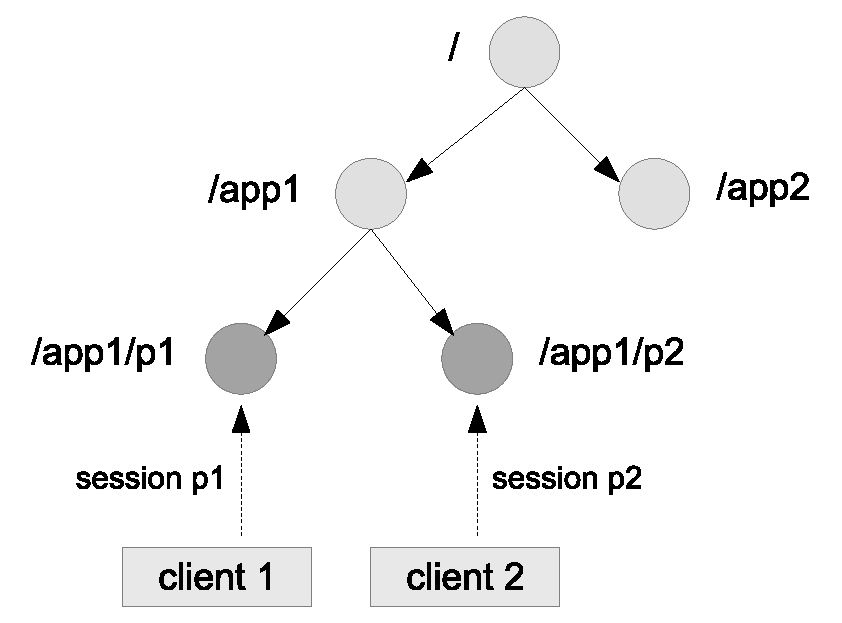
\includegraphics [width=0.5\textwidth]{images/zookeeper_tree}
  \caption{ZooKeeper tree sructure}
  \label{fig:zookeeper_tree}
\end{figure}

ZooKeeper is designed for small data warehousing, such as configuration, status and location information.
One node is usually not bigger than one kilobyte.
Therefore it stores data tree image in memory, keeping in a persistent store only transaction logs and snapshots.
In-memory storage limits the size of the database of ZooKeeper.
However, it gives advantages of low latency and high performance. 

The key feature of ZooKeeper is that it uses First In, First Out (FIFO) method for processing the messages.
It means that all commands are performed in the order they are received.
Thus, ZooKeeper maintains the total ordering.
The order is specified by a unique ZooKeeper Transaction id, that is assigned to each update.
 
ZooKeeper supports idempotent operations.
If a node should be updated, the system makes a note about the update and keeps an old and a new version of this node.
This allows client to receive the same message several times, being aware of when it can be applied.
Therefore all the write operations are performed sequentially in one thread and only on the master node.
On the contrary, read requests do not necessarily need the master node, they can be handled by a node's replica.

The client also supports the total ordering of the messages.
Hence if the client sends a write request and then a read request, the write operation is performed first.
Even if usually read operation does not need a lock, ZooKeeper strictly follows the order.
It allows to implement predictable asynchronous systems that work with ZooKeeper.

A client can watch a node.
If it sets a watch, it gets notified when the node is changed.
When the node sends this notification, it removes the watch.
In the case of connection problems between the client and the ZooKeeper server, the client receives a local notification.

ZooKeeper guarantees reliability using replication.
Its database is replicated to several nodes, one of them is a \textit{Leader} and the others are \textit{Followers}.
\textit{ZooKeeper Atomic Broadcast} (Zab) algorithm is used for managing the communication between the leader and the followers.
It synchronizes the replicas, broadcasts updates and recovers the valid state in the case of nodes crash.

Zab includes four phases: (1) Leader election, (2) Discovery, (3) Synchronization and (4) Broadcast.

1. On the first stage ZooKeeper uses any election algorithm to choose a leader.
After termination every node stores its vote locally in volatile memory.
When a node \textit{n} votes for a node \textit{n'}, \textit{n'} becomes a \textit{prospective leader} for \textit{n}.

2. On the second stage the nodes inform the prospective leader about the most recent transactions they accepted.
Thus the prospective leader knows the latest sequence af accepted transactions and can establish a new epoch.
From thit moment the previous leaders cannot perform any commits.
In the case of connection problems between a follower and a leader, the follower goes back to the stage (1) of this algorithm.

3. The leader is aware of the latests transactions history and during this stage synchronizes this information with its replicas.
This phase is also called voting phase, because it receives the votes from the nodes.
The leader performes a commit only if it receives acknowledgements from two of three followers.
At this moment the leader changes its state from \textit{prospective} to \textit{established}.

4. The nodes persist in this stage until a crash.
Every write request from a ZooKeeper client is broadcasted among the nodes.
New followers can join, receiving the transaction history from the leader.
The leader and its followers use periodic heartbeat messages for early failure detection.
If any of the nodes does nor receive a heartbeat message within a timeout, it shifts its state to \textit{election} and goes back to the first stage.

It can happened that one of the followers still has an outdated information when it receives the read request.
To avoid this problem, it is possible to make a force synchronisation with the master.
It is called the \textit{slow read}.
Evidently, if all the clients use the slow read the system looses the advantage of scaling.
Without force synchronisation ZooKeeper system scales for reads nicely. 
However, in this case the client that reads from a replica can obtain the outdated information.